\documentclass[conference]{IEEEtran}
\usepackage{graphicx}
\graphicspath{{../results/}}
\usepackage{amsmath}
\usepackage{booktabs}
\usepackage{url}
\usepackage[hidelinks]{hyperref}

\begin{document}

\title{Momentum in Levels, Reversion in Spreads:\\
A Systematic Study of U.S. Treasury Futures Curve Strategies, 2010--2026}

\author{\IEEEauthorblockN{Hong Si Wei Nicholas}
\IEEEauthorblockA{Nanyang Technological University\\
Singapore}}

\maketitle

\begin{abstract}
We evaluate systematic momentum and curve mean-reversion strategies on U.S.
Treasury futures over January 2010 to July 2026 using Bloomberg data. Continuous,
back-adjusted futures are reconstructed from the exchange roll map, and curve
trades are hedged to be DV01-neutral. Our central finding is a clear asymmetry
between levels and spreads: outright duration exhibits trend, so a time-series
momentum strategy earns a net Sharpe ratio of 0.68, whereas the yield-curve
slope exhibits mean-reversion. A naive momentum signal applied to the 2s10s
slope is empirically duration-neutral yet loses money (net Sharpe $-0.79$),
while the same book driven by a mean-reversion signal earns 0.71. Two curve
mean-reversion strategies (2s10s and 5s30s) perform comparably to the
outright-momentum baseline but do not statistically dominate it, and a
2s5s10s butterfly does not earn its risk. All results are net of transaction
costs and scaled to a common volatility target. We discuss the methodological
requirements---roll reconstruction, DV01 hedging, and leakage-free
backtesting---that materially affect these conclusions, and we are explicit
about the out-of-sample validation still required before the curve results can
be treated as a hard performance claim.
\end{abstract}

\begin{IEEEkeywords}
fixed income, Treasury futures, time-series momentum, mean-reversion, yield
curve, systematic strategies, backtesting.
\end{IEEEkeywords}

\section{Introduction}
Systematic strategies in fixed income are commonly organized around three
premia: carry, momentum, and value/mean-reversion. Time-series momentum has
been documented across asset classes~\cite{tsmom}, and carry has been shown to
be a broadly compensated factor~\cite{carry}. Fixed-income practitioners have
long distinguished \emph{outright} directional exposure (the level of rates)
from \emph{relative-value} curve exposure (the slope and curvature between
maturities)~\cite{ilmanen}. These two exposures need not share the same
time-series behavior, and conflating them---for example, applying a single
momentum overlay to both---can be actively harmful.

This paper makes that distinction concrete on the most liquid expression of the
U.S. rates market, CME Treasury futures. We study the momentum and
mean-reversion premia only; carry is outside the scope of this paper. We construct a reproducible pipeline
that (i) rebuilds continuous futures from the exchange roll map, (ii) hedges
curve trades to DV01 neutrality, and (iii) backtests a small, pre-specified set
of strategies under a leakage-free protocol. Our contribution is not a new
signal but a clean, honestly-reported empirical contrast: over 2010--2026,
outright duration trends while the curve mean-reverts, and we quantify the cost
of getting that distinction wrong.

\section{Data}
All series are daily Bloomberg exports covering January 2010 to July 2026,
inner-joined onto the trading calendar of the front 10-year note future,
yielding approximately 4{,}160 observations. The dataset comprises: the
constant-maturity cash Treasury curve (3M, 6M, 1Y, 2Y, 3Y, 5Y, 7Y, 10Y, 20Y,
30Y); the SOFR/OIS and (legacy) swap curves together with Fed funds futures and
the policy target rate for the macro overlay; and the futures complex itself
across six roots---2Y (ZT), 5Y (ZF), 10Y (ZN), Ultra 10Y (TN), classic Bond
(ZB), and Ultra Bond (UB)---each with the first three generic contracts and
per-contract static specifications. The MOVE index, VIX, and 10-year breakeven
inflation complete the volatility and macro controls.

Three data-handling issues materially affect correctness and are addressed
explicitly in the pipeline. First, Bloomberg stamps prior values on
non-trading days in the cash index series; the inner join to the futures
calendar removes these phantom rows. Second, contract-level date fields are
returned as locale-dependent text, which can silently transpose day and month;
these are parsed day-first and validated against the futures month code.
Third, and most importantly for return construction, the mapping from each
generic to its underlying contract is retained so that rolls can be identified
and neutralized rather than contaminating returns.

\section{Methodology}

\subsection{Continuous futures}
For each root we take the front generic's settlement series and identify roll
dates as changes in the underlying-contract identifier. We then apply a
difference back-adjustment: the settlement gap introduced on each roll date is
treated as a contract switch rather than a price move, and the cumulative sum of
all \emph{future} roll gaps is subtracted from each historical level. The
resulting series has no artificial roll jumps, and daily returns are computed
from the adjusted level.

\subsection{DV01-neutral hedging}
Curve trades require the two (or three) legs to be balanced in interest-rate
sensitivity. We use each contract's daily forward DV01 as published by Bloomberg
(the risk to delivery of the cheapest-to-deliver bond, adjusted by its conversion
factor), taken as a time series over the full sample. The hedge ratio for a spread
is the ratio of the two legs' DV01s, lagged one day. This holds the realized books
duration-neutral: the regression of the 2s10s book's daily P\&L on the 10-year
yield change has a slope of $-0.001$, indistinguishable from zero. Using the
contract's own forward risk avoids the estimation noise and lag of a
regression-based DV01 proxy, particularly around delivery and cheapest-to-deliver
switches.

\subsection{Signals}
Two signal families are used, each matched to the exposure it drives:
\begin{itemize}
\item \textbf{Outright duration (momentum).} The sign of the trailing 63-day
return of each root's continuous series.
\item \textbf{Curve (mean-reversion).} The negative standardized deviation of
the relevant spread (2s10s, 5s30s) or curvature (2s5s10s) from its own
trailing 252-day mean, clipped at $\pm 3$ and lagged one day.
\end{itemize}
The choice of mean-reversion for the curve is motivated economically---slopes
and spreads are stationary relative to levels---and is examined empirically in
Section~\ref{sec:results}.

\subsection{Backtest protocol}
Positions are formed from information available at $t{-}1$ and executed at the
$t$ settlement. Rebalancing is monthly. Each book is scaled toward a 10\%
annualized volatility target using 63-day realized volatility, with leverage
capped at $3\times$ and a 126-day warm-up before any position is taken, so that
a small early-sample volatility estimate cannot inflate the book. Transaction
costs are charged at one tick per contract per side, using the per-contract tick
size from the static specifications (the 10-year tick, for example, was halved
over the sample, which the per-contract data captures).

\subsection{Evaluation}
We report the annualized Sharpe ratio (net of costs), maximum drawdown, and
annual turnover. To compare each strategy against the outright-momentum baseline
we use the Diebold--Mariano test~\cite{dm} on the daily net-return differential.
Because positions are rebalanced monthly, a holding is carried for roughly
twenty-one trading days and the daily return differentials are strongly
autocorrelated; we therefore estimate the long-run variance with a Newey--West
(Bartlett-kernel) HAC estimator at a lag spanning the monthly holding, and apply
the Harvey--Leybourne--Newbold small-sample correction with Student-$t$ critical
values. A positive statistic means the alternative out-returns the baseline. We
verified the implementation against a HAC-robust regression of the differential
on a constant.

\section{Results}
\label{sec:results}

\subsection{The level--spread asymmetry}
The paper's central result is summarized in Fig.~\ref{fig:signal}. The 2s10s
book is constructed identically in both lines---long the 10-year leg, short a
DV01-scaled 2-year leg---and differs only in the signal that sizes it. Driven
by momentum, the book returns a net Sharpe of $-0.79$; driven by
mean-reversion, it returns $0.71$. Because the book is empirically
duration-neutral, this gap is not a hedging artifact: it reflects the curve's
tendency to revert rather than trend. Applying the outright-momentum recipe to
the curve is, over this sample, a systematic way to lose money.

\begin{figure}[t]
\centering
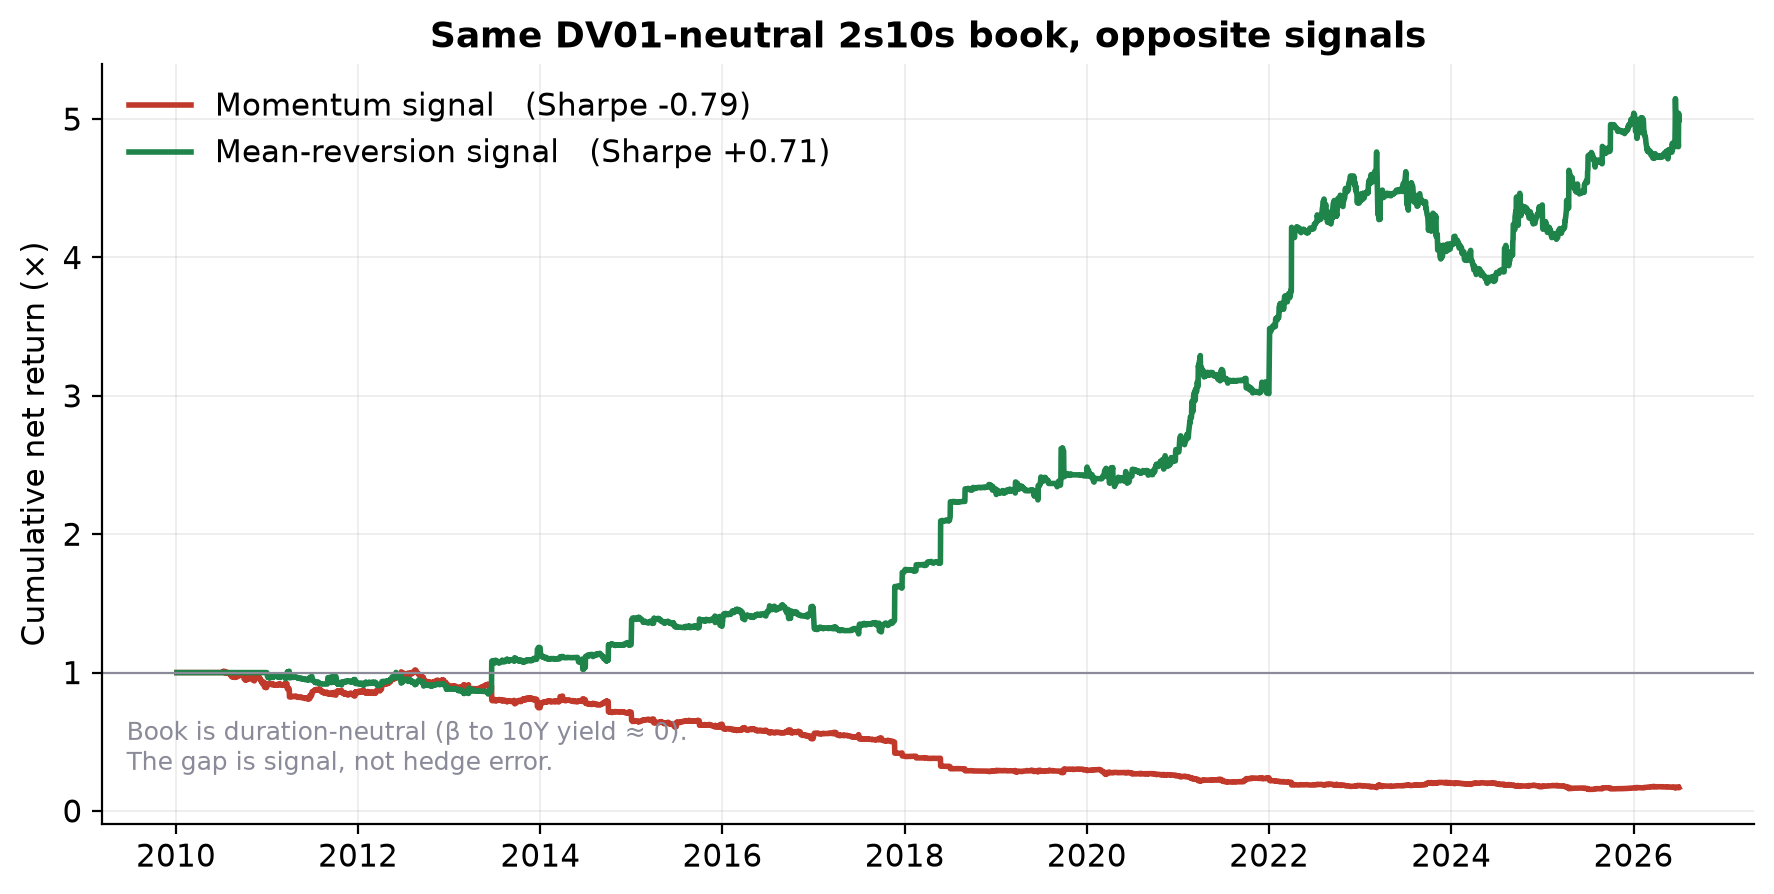
\includegraphics[width=\columnwidth]{fig1_signal_contrast.png}
\caption{The 2s10s DV01-neutral book under two signals. The book is identical;
only the signal differs. Momentum loses (net Sharpe $-0.79$); mean-reversion
earns (net Sharpe $0.71$). The book's P\&L has near-zero sensitivity to the
10-year yield, so the difference is signal, not hedge error.}
\label{fig:signal}
\end{figure}

\subsection{Strategy performance}
Table~\ref{tab:results} reports the four pre-specified strategies with the
signal appropriate to each exposure, and Fig.~\ref{fig:equity} shows their net
cumulative performance. Outright duration momentum and the two curve
mean-reversion trades cluster in a Sharpe range of $0.66$ to $0.71$ with
drawdowns of roughly 20--27\%. The 2s5s10s butterfly is weak (Sharpe $0.07$) and
carries the largest drawdown; on the evidence here it does not earn its place.

\begin{table}[t]
\caption{Net-of-cost performance, 2010--2026}
\label{tab:results}
\centering
\begin{tabular}{lccc}
\toprule
Strategy & Sharpe & Max DD & Turnover/yr \\
\midrule
Duration momentum (baseline) & 0.68 & $-23\%$ & 22 \\
2s10s mean-reversion         & 0.71 & $-20\%$ & 104 \\
5s30s mean-reversion         & 0.66 & $-27\%$ & 68 \\
2s5s10s butterfly            & 0.07 & $-38\%$ & 87 \\
\bottomrule
\end{tabular}
\end{table}

\begin{figure}[t]
\centering
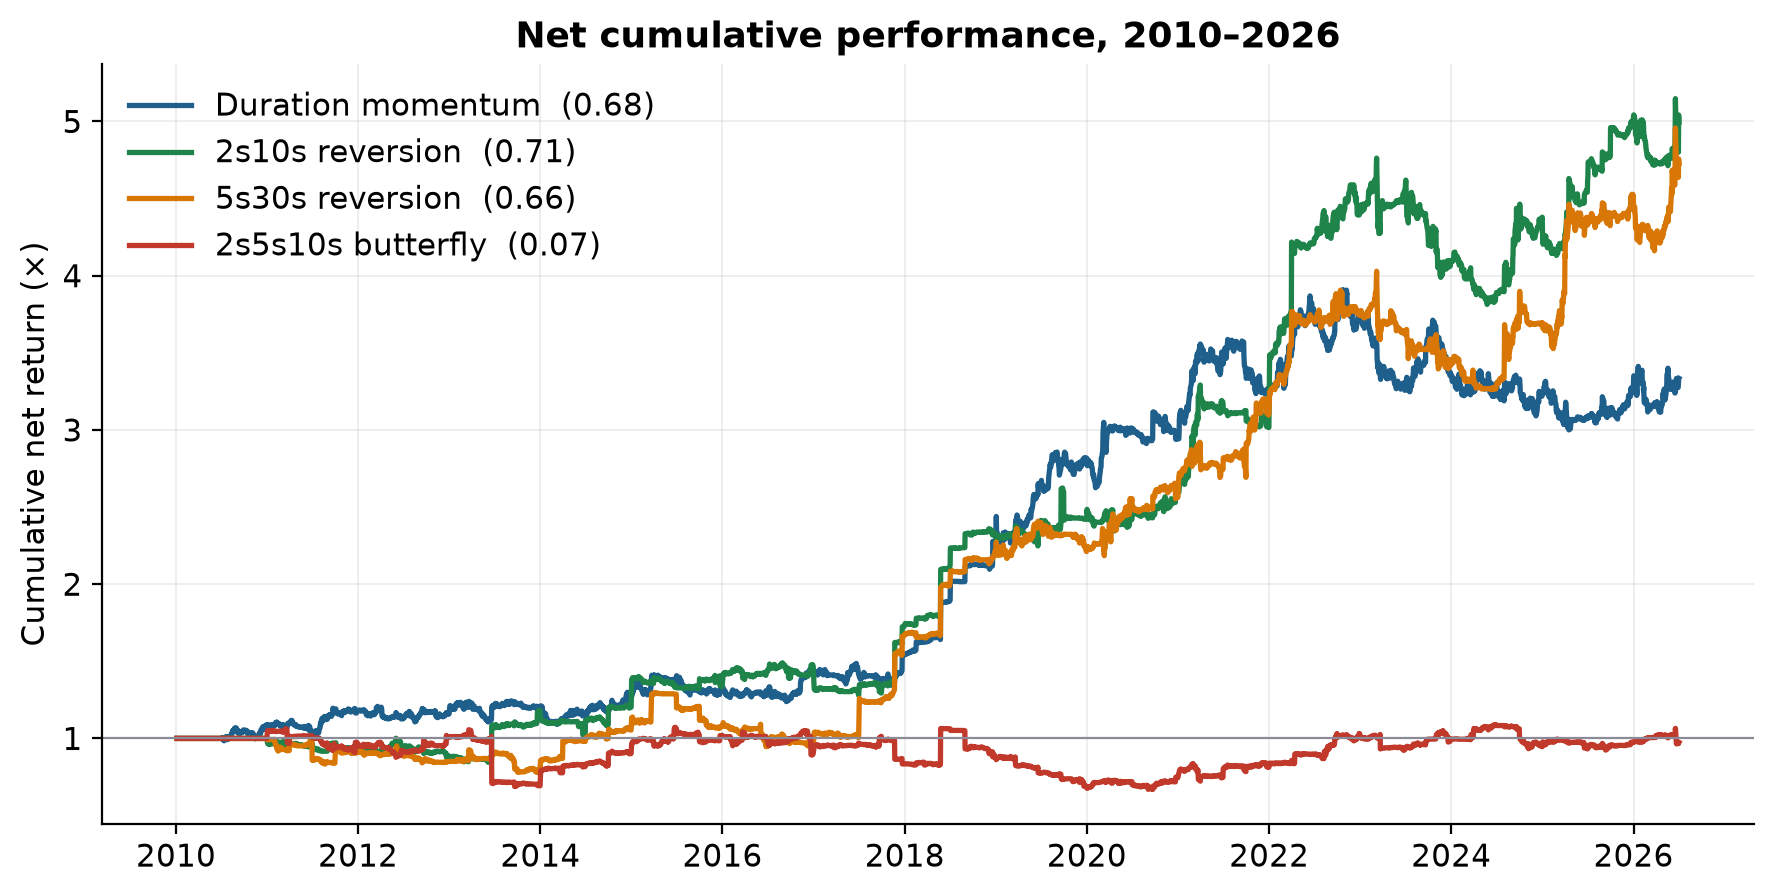
\includegraphics[width=\columnwidth]{fig2_equity_curves.png}
\caption{Net cumulative performance of the four strategies, volatility-scaled
and after transaction costs. The three viable strategies advance broadly
together; the butterfly is flat to negative.}
\label{fig:equity}
\end{figure}

\subsection{Does the curve add to the baseline?}
Relative to the outright-momentum baseline, the HAC Diebold--Mariano statistics
for the 2s10s and 5s30s mean-reversion trades are positive but small
($\mathrm{DM}=0.83$, $p=0.41$ and $\mathrm{DM}=0.68$, $p=0.49$), corresponding to
an annualized return edge of about $2.9\%$ and $2.7\%$ that is not statistically
distinguishable from zero; the butterfly is negative ($\mathrm{DM}=-1.53$,
$p=0.13$). We therefore do not claim that the curve trades outperform the
baseline: they are
comparable but not statistically distinguishable from it under this test. The
honest reading is that outright duration momentum is the workhorse, curve
mean-reversion is a legitimate and roughly co-equal source of return, and the
butterfly is not supported.

\subsection{Macro regime overlay}
As a control and as an exportable input to a separate FX-volatility project, we
classify each day into a coarse regime from the MOVE z-score and the level and
trailing change of the 2s10s slope, yielding a stress state (771 days), a
steepening state (1{,}454 days), and a flattening state (1{,}948 days). We
report this as a descriptive conditioning variable; extending it into a
real-time signal would require out-of-sample validation of its own.

\section{Discussion and Limitations}
Two caveats bound the strength of these conclusions. \emph{First}, the decision
to use mean-reversion rather than momentum for the curve is economically
motivated but was confirmed on the full sample; a single full-sample sign is not
proof, and a walk-forward, out-of-sample test is required before the curve
results are treated as a hard performance claim. \emph{Second}, the study is
single-country and single-currency; the cost model, while contract-specific, is
a flat tick-per-side approximation that omits market impact and financing.
Neither is expected to reverse the qualitative level-versus-spread finding, but
the out-of-sample validation of the curve-signal direction is the dominant open
item and is what would move the curve results from suggestive to established.

\section{Conclusion}
On U.S. Treasury futures over 2010--2026, outright duration trends and the yield
curve mean-reverts. A momentum overlay that is correct for the former is
actively wrong for the latter: an identically-hedged, duration-neutral 2s10s
book loses at a Sharpe of $-0.79$ under momentum and earns $0.71$ under
mean-reversion. Matching each signal to its exposure yields three viable
strategies near a Sharpe of $0.7$; the curve trades are comparable to, but do
not dominate, the outright-momentum baseline, and a butterfly is not supported.
The result underscores that in fixed income the construction details---roll
reconstruction, DV01 hedging, and signal--exposure matching---are not
incidental but decisive.

\begin{thebibliography}{1}
\bibitem{tsmom} T. J. Moskowitz, Y. H. Ooi, and L. H. Pedersen, ``Time series
momentum,'' \emph{Journal of Financial Economics}, vol. 104, no. 2,
pp. 228--250, 2012.
\bibitem{carry} R. S. J. Koijen, T. J. Moskowitz, L. H. Pedersen, and E. B.
Vrugt, ``Carry,'' \emph{Journal of Financial Economics}, vol. 127, no. 2,
pp. 197--225, 2018.
\bibitem{ilmanen} A. Ilmanen, \emph{Expected Returns: An Investor's Guide to
Harvesting Market Rewards}. Chichester, U.K.: Wiley, 2011.
\bibitem{dm} F. X. Diebold and R. S. Mariano, ``Comparing predictive
accuracy,'' \emph{Journal of Business \& Economic Statistics}, vol. 13, no. 3,
pp. 253--263, 1995.
\bibitem{gsw} R. S. G\"urkaynak, B. Sack, and J. H. Wright, ``The U.S. Treasury
yield curve: 1961 to the present,'' \emph{Journal of Monetary Economics},
vol. 54, no. 8, pp. 2291--2304, 2007.
\end{thebibliography}

\end{document}
